\documentclass[11pt,a4paper]{article}

\usepackage[utf8]{inputenc}
\usepackage[T1]{fontenc}
\usepackage[english]{babel}
\usepackage{amsmath,amssymb}
\usepackage{siunitx}
\sisetup{detect-all, per-mode=symbol}
\usepackage{booktabs}
\usepackage{array}
\usepackage{graphicx}
\usepackage[section]{placeins}
\newcolumntype{L}[1]{>{\raggedright\arraybackslash}p{#1}}
\usepackage{microtype}
\setlength{\emergencystretch}{2em}
\usepackage[margin=2.5cm]{geometry}
\usepackage{xcolor}
\definecolor{darkblue}{HTML}{1F4E79}
\usepackage[colorlinks=true,linkcolor=darkblue,citecolor=darkblue,urlcolor=darkblue]{hyperref}

\graphicspath{{figuras/}}

\title{Damping versus oscillations in the setting of Hadžić, Rein,\\ Schrecker and Straub\\[0.3em]
       \large Loop gain, linear theory and particle-in-cell runs}
\author{Working notes}
\date{3 October 2026}

\begin{document}
\maketitle

\begin{abstract}
Hadžić, Rein, Schrecker and Straub proved that, in the radial Vlasov--Poisson system with
a central point mass and all particles at the same angular momentum, small steady states
$\varepsilon(E_t-E)^k$ damp their linear perturbations if $k>1$ and do not if
$1/2<k\le1$, because a discrete eigenvalue appears below the band of orbital frequencies.
The theorem holds below a mass $\varepsilon_0(k)$ that it does not estimate. We reproduce
their setting with our tools and study it at finite mass. The criterion for the discrete
mode is that the gain $\lambda_{\rm edge}$ of the self-consistent loop at the lower edge of
the band exceeds one; $\lambda_{\rm edge}$ is the norm of the Mathur operator of their
proof. At small mass ($a_0=0.01$) $\lambda_{\rm edge}\approx0.02$ for $k>1$ and diverges
for $k\le1$, as the theorem requires, but the discrete mode of $k\le1$ lies less than
$10^{-6}$ band widths below the edge. The threshold $\lambda_{\rm edge}=1$ is reached at
$a_0\approx0.53$ for $k=1.25$ and $a_0\approx0.93$ for $k=1.5$; for $k=2$ and $3$ there is
no discrete mode even with a shell as massive as the central mass. In these units the
coupling parameter $\eta$ of our earlier work is $1.25$ and $2.6$ at the two thresholds,
and above $3$ for $k=2$: $\eta$ does not mark the transition, $\lambda_{\rm edge}$ does. The
linearized solver confirms all of this in time. Particle-in-cell runs with $10^4$ particles
follow linear theory to \SI{1}{\%} up to $t\approx1000$ at small mass; at $a_0=1$ they show the
undamped mode of $k=0.75$ and $k=1$ at the predicted frequency (to about $10^{-3}$) and the
Landau damping of $k=2$ at the predicted rate (to \SI{5}{\%}). The modes that lie just below
the edge ($k=1.25$ and $1.5$) lose amplitude in the runs. A scan in amplitude, grid and
number of particles shows that this loss is a finite-amplitude effect: it grows with
$\varepsilon$ and does not change with $\Delta r$ or $N$. With $4\times10^4$ particles the mode of
$k=1.25$ persists up to $t=4000$ at the predicted frequency. The departure of the reference
runs from stationarity has two parts: an initial level set by the grid, and a later growth
caused by the discreteness of the particles, which four times more particles remove.
\end{abstract}

\tableofcontents

\section{Model and theory}
\label{sec:teoria}

\subsection{The setting of the theorem}

We consider the radial Vlasov--Poisson system in which all particles have the same
modulus of angular momentum $L_0$, around a point mass $M=1$ (with $G=1$),
\[
  \partial_tF+p_r\,\partial_rF-\partial_r\Phi_{\rm ef}\,\partial_{p_r}F=0,\qquad
  \Phi_{\rm ef}=-\frac1r+\Phi_{\rm self}+\frac{L_0^2}{2r^2},
\]
where $\Phi_{\rm self}$ is the potential of the density $4\pi r^2\rho=8\pi^2L_0\int F\,dp_r$.
This is the system of Hadžić, Rein, Schrecker and Straub [HRSS], with their squared
angular momentum $L=L_0^2$. We use $L_0=2$, so that the circular orbit of the bare point
mass is at $r=4$ with energy $E_{\min}=-1/8$, and the radial frequency is
$\Omega(J)=(J+2)^{-3}$ without self-gravity.

The steady states are polytropes in the energy,
\[
  F_{\rm eq}=A\,(E_t-E)^k\quad(E<E_t),\qquad F_{\rm eq}=0\quad(E\ge E_t),
\]
where $k$ is the exponent of the vacuum edge and $E_t=E(J_t)$ is the energy of the orbit
of action $J_t$, the edge of the support. We use $J_t=0.7$. Without self-gravity this gives
$E_t=-0.0686$, within their single-gap condition $-2^{-2/3}/8=-0.079<E_t<0$, which
requires $\Omega_{\max}\ge2\,\Omega_{\min}$; here $\Omega_{\max}/\Omega_{\min}=2.46$. The bands of the
harmonics $n=1,2,\dots$ then overlap, and the only gap in the spectrum is the principal
one, $(0,\Omega_{\min})$. The mass $a_0$ of the shell is measured in units of the central
mass; their small parameter $\varepsilon$ is proportional to it.

\subsection{The theorem}

For $k>1/2$ and $\varepsilon$ below a threshold $\varepsilon_0(k)$ [HRSS, Thm.~1.2]:
\begin{itemize}
\item if $1/2<k\le1$ the linearized operator has an eigenvalue in the principal gap, so the
perturbation does not damp; this includes the King model;
\item if $k>1$ the point spectrum is empty and the field damps in the time-averaged sense
$\lim_{T\to\infty}T^{-1}\int_0^T\|\nabla U\|^2dt=0$, without a rate.
\end{itemize}
The value of $\varepsilon_0(k)$ is not estimated. The proof uses a Birman--Schwinger principle
due to Mathur: there is an eigenvalue in the gap if and only if the norm of the Mathur
operator $M_\lambda$ is at least one for some $\lambda$ in the gap. For $k>1$ they show
$M_\lambda\le C\varepsilon$, and for $k\le1$ that $M_\lambda$ diverges at the edge of the gap.

\subsection{The loop gain}
\label{sec:lazo}

In angle--action variables a mode $\delta F=a(Q,J)e^{-i\omega t}$ obeys, harmonic by
harmonic, $(k\Omega-\omega)a_k=kF_{\rm eq}'(J)\,\delta\Phi_k(J)$, where $\delta\Phi_k$ is the
harmonic of the potential along the orbit $J$. (Here $k$ is a Fourier index; the edge
exponent is also called $k$, following [HRSS], and the context distinguishes them.) The
density sees only the part of $\delta F$ even in $Q$, and with $b_k=a_k+a_{-k}$,
\[
  b_k=R_k\,\delta\Phi_k,\qquad R_k(J;\omega)=\frac{2k^2\Omega F_{\rm eq}'}{k^2\Omega^2-\omega^2},
\]
while the Poisson equation gives
\begin{gather*}
  \delta\Phi_k=\sum_{k'}\int M_{kk'}(J,J')\,b_{k'}\,dJ',\\
  M_{kk'}=4\pi L_0\iint\cos kQ\,\cos k'Q'\,G\big(r(Q,J),r(Q',J')\big)\,dQ\,dQ',
\end{gather*}
with $G=-1/\max(r,r')$.
A mode exists if $MR(\omega)$ has the eigenvalue one. For $F_{\rm eq}'<0$ and $\omega<\Omega_{\min}$
this operator is similar to the symmetric positive operator $|R|^{1/2}(-M)|R|^{1/2}$; its
largest eigenvalue $\lambda(\omega)$ is the gain of the loop potential $\to$ density $\to$
potential, and $\lambda_{\rm edge}=\lambda(\Omega_{\min})$. Since $\lambda$ grows with $\omega$ and
$\lambda(0)<1$ (Antonov),
\[
  \text{there is a discrete mode below the band}\iff\lambda_{\rm edge}>1,
\]
and its frequency $\omega_d$ is the root of $\lambda(\omega_d)=1$. $\lambda(\omega)$ is the norm of
the Mathur operator with $\lambda_{\rm Mathur}=\omega^2$. Near the edge
$|R_1|\propto(J_t-J)^{k-1}/(\Omega-\omega)$, so $\lambda_{\rm edge}$ is finite only for $k>1$. We
write $\delta_d=(\Omega_{\min}-\omega_d)/\Delta\Omega$ for the distance of the mode below the
edge in band widths. The derivation is in Section~1.5 of the demo document
(\texttt{docs/demo\_eta/demo\_eta.pdf}).

\subsection{The coupling parameter \texorpdfstring{$\eta$}{eta}}

In earlier work we used $\eta=\delta\Omega/(\Delta\Omega/\bar\Omega)$, the self-gravitational shift
of the mass-weighted mean frequency, $\delta\Omega=(\bar\Omega-\bar\Omega_0)/\bar\Omega_0$, divided by the
relative width of the band; $\bar\Omega_0$ is the same average for the same distribution
without self-gravity. $\eta$ needs only the equilibrium. Here we compare it with
$\lambda_{\rm edge}$.

\section{Numerical methods}
\label{sec:metodos}

\subsection{Equilibria}

The equilibria are built by fixed-point iteration (\texttt{equilibrio.py} with
\texttt{-{}-fondo puntual -{}-forma polE}): the angle--action map of the total potential,
the table $E(J)$, the polytrope with $E_t=E(J_t)$ recomputed at each iteration, the density
and the Poisson equation, until the potential changes by less than $10^{-13}$. The
iteration converges in 6--42 iterations for $0.01\le a_0\le1$. With the bare point mass the
map gives $J(E)=1/\sqrt{-2E}-2$ to $1.7\times10^{-15}$ and the circular orbit at
$r=4.000015$. The option is neutral for the isochrone used before: the equilibria,
initial states and linear solutions of earlier runs are reproduced bit for bit.

\subsection{Loop gain and linear solver}

$\lambda(\omega)$ is computed by \texttt{lambda\_borde.py}: $J=J_t(1-s^2)$ with 200
Gauss--Legendre nodes in $s$, 128 points in $Q$, harmonics up to $k=6$, and the integrals
in $Q$ on a radial grid of 2000 nodes, so that $M=4\pi L_0\,PGP^{\rm T}$. In this setting,
doubling the resolution changes $\lambda_{\rm edge}$ by at most $2\times10^{-4}$ for $k=2$ and
$3\times10^{-3}$ for $k=1.25$. For $k\le1$, $\lambda$ diverges at the edge and its value on
the grid grows with the resolution; the frequency $\omega_d$ is converged.

The linearized solver (\texttt{lineal.py}) integrates the linear equation in time on
$1600\times32$ nodes in $(J,Q)$ with $\Delta t=0.5$, from the initial perturbation
$\delta F=F_{\rm eq}(J/J_t)^{3/2}\cos Q$. The observable is
\[
  h_1(t)=\frac{\sum\delta F\,B(J)\,e^{-iQ}}{\sum F_{\rm eq}B(J)},\qquad
  B(J)=J^2e^{-(J-0.35)^2/0.2^2},
\]
and $\|\delta\Phi\|$ is the rms value of $\delta\Phi$ over the radii of the shell.

\subsection{PIC runs}

The PIC code (\texttt{VP\_PIC}) uses \texttt{BGtype = sphere}, a uniform ball of mass 1 and
radius 1: for $r>1$ it is the point mass, and the shells lie at $1.8<r<12.2$. Each run has
$400\times25=10^4$ particles on a regular grid in the angle--action variables of the
equilibrium, $\Delta r=0.1$ on $[0,20]$, the fourth-order Yoshida integrator and
$\Delta t=0.1$ (Courant factor 2). Each perturbed run (D) has a reference run (Z) with the
same particles and $\varepsilon=0$; the perturbation is $(h_{1,D}-h_{1,Z})/\varepsilon$, and
the same for $\delta\Phi$. $h_1$ is computed with the angle--action map of the equilibrium.
Table~\ref{tab:corridas} lists the runs.

\begin{table}[!htbp]
\centering
\small
\begin{tabular}{lL{2.6cm}lL{2.2cm}L{2.2cm}L{3.2cm}}
\toprule
series & $k$ & $a_0$ & $\varepsilon$ & $t_{\rm fin}$, output & purpose\\
\midrule
1 & 0.75, 1, 1.5, 2 & 0.01 & 0.1 (and Z) & 8000, every 20 & the regime of the theorem\\
2 & 0.75, 1, 1.25, 1.5, 2 & 1 & 0.1 (and Z) & 4000, every 5 & bound modes and the threshold\\
3 & 0.75, 1, 1.5, 2 & 0.01 & 0.5 (Z of series 1) & 8000, every 20 & a lower floor\\
4 & 1.25, 1.5 & 1 & 0.03, 0.3 (Z of series 2); 0.1 with $\Delta r/2$ or $4N$ (and Z) & 4000, every 5 & amplitude, grid and particles (Section~\ref{sec:borde})\\
\bottomrule
\end{tabular}
\caption{The 34 PIC runs. Each takes \SIrange{220}{380}{s} with four threads, and
\SIrange{840}{860}{s} with $4\times10^4$ particles. The energy is conserved to
$|\Delta E/E|\le1.3\times10^{-7}$ at $a_0=0.01$ and $\le1.8\times10^{-5}$ at $a_0=1$.}
\label{tab:corridas}
\end{table}

\section{Results}
\label{sec:resultados}

\subsection{The loop gain and the threshold mass}

Table~\ref{tab:lambda} and Figure~\ref{fig:lambda} give $\lambda_{\rm edge}$ for 36 equilibria.

\begin{table}[!htbp]
\centering
\small
\begin{tabular}{lrrrrrr}
\toprule
$k$ \textbackslash\ $a_0$ & 0.01 & 0.03 & 0.1 & 0.3 & 0.6 & 1.0\\
\midrule
0.75 & $\infty$ & $\infty$ & $\infty$ & $\infty$ & $\infty$ & $\infty$\\
 & ($<10^{-6}$) & ($2\times10^{-6}$) & ($10^{-4}$) & (0.004) & (0.027) & (0.075)\\
1 & $\infty$ & $\infty$ & $\infty$ & $\infty$ & $\infty$ & $\infty$\\
 & ($<10^{-6}$) & ($<10^{-6}$) & ($<10^{-6}$) & (0.0002) & (0.0085) & (0.044)\\
1.25 & 0.025 & 0.075 & 0.240 & 0.643 & 1.112 & 1.558\\
 & & & & & (0.0001) & (0.019)\\
1.5 & 0.018 & 0.054 & 0.170 & 0.448 & 0.759 & 1.050\\
 & & & & & & (0.0015)\\
2 & 0.016 & 0.046 & 0.145 & 0.371 & 0.609 & 0.820\\
3 & 0.016 & 0.047 & 0.145 & 0.358 & 0.567 & 0.738\\
\bottomrule
\end{tabular}
\caption{$\lambda_{\rm edge}$ and, in parentheses, the distance $\delta_d$ of the discrete mode below
the edge in band widths, where there is a mode. For $k\le1$, $\lambda_{\rm edge}=\infty$.}
\label{tab:lambda}
\end{table}

\begin{figure}[htbp]
\centering
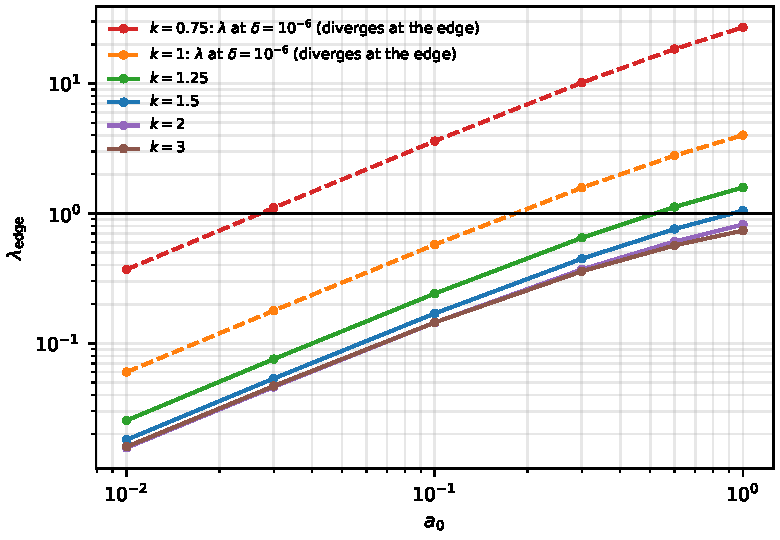
\includegraphics[width=0.7\textwidth]{lambda_mapa.pdf}
\caption{$\lambda_{\rm edge}$ against the mass for $k>1$ (solid). For $k\le1$, where it
diverges, the dashed lines show $\lambda$ at $10^{-6}$ band widths below the edge. A
discrete mode exists above the horizontal line.}
\label{fig:lambda}
\end{figure}

\begin{itemize}
\item \textbf{The theorem at small mass.} For $k>1$, $\lambda_{\rm edge}$ is proportional to the
mass, $0.016$--$0.025$ at $a_0=0.01$, as their bound $M_\lambda\le C\varepsilon$ says. For $k\le1$,
$\lambda$ diverges at the edge, as $\ln(1/\delta)$ for $k=1$ and as a power for $k=0.75$, so there
is always a mode. At small mass it is bound by less than $10^{-6}$ band widths.
\item \textbf{The threshold $\varepsilon_0(k)$.} Interpolating $\lambda_{\rm edge}=1$, the mode
appears at $a_0\approx0.53$ for $k=1.25$ and $a_0\approx0.93$ for $k=1.5$. For $k=2$ and $3$
there is no mode up to $a_0=1$, where $\lambda_{\rm edge}=0.82$ and $0.74$.
\item \textbf{Their hypotheses.} $\Omega(J)$ is monotonic in all 36 equilibria. The single-gap
condition $\Omega_{\max}/\Omega_{\min}\ge2$ holds up to $a_0=0.3$; it is lost at $a_0=0.6$ for $k=0.75$
($1.99$) and at $a_0=1$ for $k\le1.5$ ($1.87$--$1.98$).
\end{itemize}

\subsection{The coupling parameter \texorpdfstring{$\eta$}{eta}}

\begin{table}[!htbp]
\centering
\small
\begin{tabular}{lrrrrrr}
\toprule
$k$ \textbackslash\ $a_0$ & 0.01 & 0.03 & 0.1 & 0.3 & 0.6 & 1.0\\
\midrule
0.75 & 0.015 & 0.045 & 0.160 & 0.558 & 1.334 & 2.668\\
1 & 0.016 & 0.048 & 0.169 & 0.586 & 1.388 & 2.748\\
1.25 & 0.017 & 0.051 & 0.178 & 0.613 & 1.437 & 2.818\\
1.5 & 0.017 & 0.053 & 0.187 & 0.637 & 1.481 & 2.883\\
2 & 0.019 & 0.058 & 0.202 & 0.680 & 1.560 & 2.997\\
3 & 0.022 & 0.066 & 0.227 & 0.751 & 1.686 & 3.182\\
\bottomrule
\end{tabular}
\caption{$\eta$ of the same equilibria. The relative width of the band is $0.57$--$0.80$,
against $0.16$--$0.29$ in the isochrone of our earlier work.}
\label{tab:eta}
\end{table}

$\eta$ is $0.015$--$0.022$ at $a_0=0.01$, the regime of the theorem (Table~\ref{tab:eta}).
At the threshold it is $\eta\approx1.25$ for $k=1.25$ and $\eta\approx2.6$ for $k=1.5$, and
$\eta=3.0$ is not enough for $k=2$. In the isochrone the Wilson model ($k=2$) had its threshold
at $\eta\approx1.18$. With a band this wide the shape of the edge weighs more in the
coupling than the shift of the mean frequency, and $\eta$ does not mark the transition. The
criterion $\lambda_{\rm edge}=1$ is the same for every $k$.

\subsection{Linear response in time}

At $a_0=0.01$ the linear response decays algebraically for every $k$. The slope of the
envelope of $|h_1|$ against $\ln t$ over $1000\le t\le8000$ is $-1.67$, $-2.00$, $-2.55$ and
$-3.00$ for $k=0.75$, $1$, $1.5$ and $2$, close to $t^{-(k+1)}$, the tail of an edge at which
the weight vanishes as $(J_t-J)^k$. The sharper the edge, the slower the decay. For $k\le1$
the discrete mode is too weakly bound to appear in this time.

At $a_0=1$ (Figure~\ref{fig:a1}, black) the solver confirms the loop gain in time. For
$k=0.75$, $1$ and $1.25$, $|h_1|$ levels off at $0.075$, $0.071$ and $0.059$, and oscillates at
$0.14169$, $0.14783$ and $0.15330$, against $\omega_d=0.14169$, $0.14785$ and $0.15326$ from
$\lambda(\omega_d)=1$. For $k=1.5$, with the mode $0.0015$ band widths below the edge, it decays
slowly towards a plateau ($0.022$ at $t=4000$) and oscillates at $0.1574$ against $0.15751$.
For $k=2$ it is damped: the fitted pole is $\omega=0.1663$--$0.1669$, inside the band, with
$\gamma=6.4$--$6.5\times10^{-3}$, and $|h_1|$ falls to $10^{-5}$ by $t=4000$.

\subsection{PIC runs at small mass}

\begin{figure}[htbp]
\centering
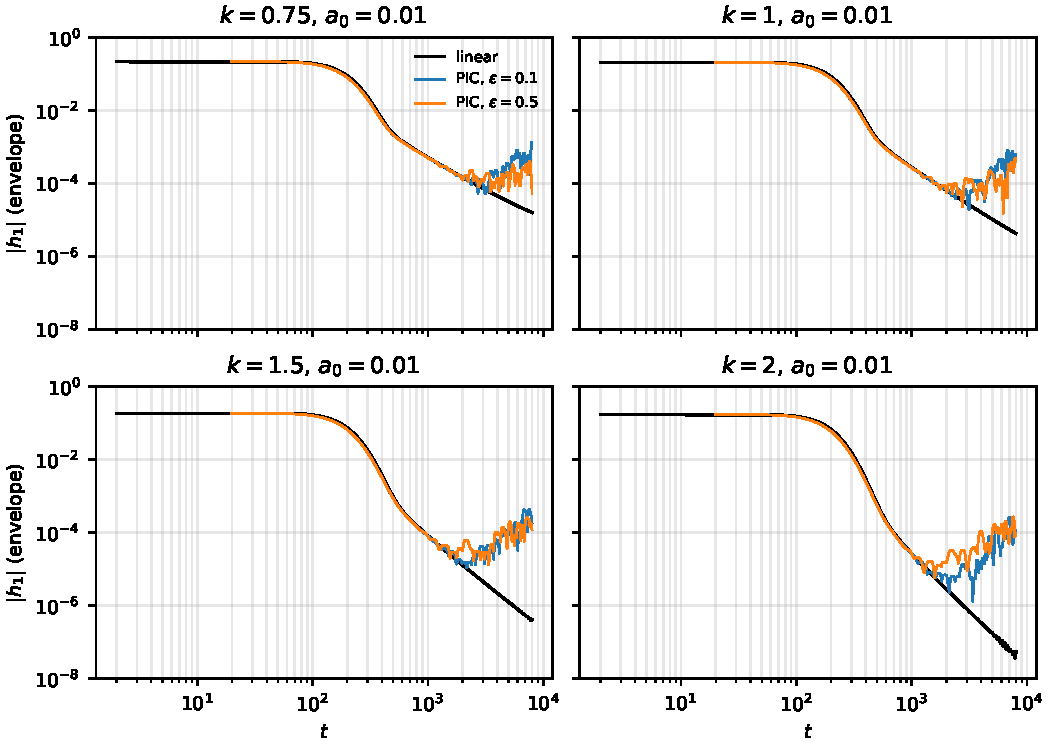
\includegraphics[width=0.9\textwidth]{pic_a001.pdf}
\caption{$a_0=0.01$: envelope of $|h_1|$ in linear theory (black) and in the PIC runs with
$\varepsilon=0.1$ (blue) and $\varepsilon=0.5$ (orange).}
\label{fig:a001}
\end{figure}

The PIC runs follow linear theory to \SI{1}{\%} in $|h_1|$ up to $t\approx1000$ (12
$\tau_1$, with $\tau_1=2\pi/\Delta\Omega=84$), except $k=2$ (\SI{5}{\%}). After that they reach a
floor (Figure~\ref{fig:a001}): the D and Z runs decorrelate, and at $t\approx8000$ their
difference is of the order of the noise of the unperturbed run itself. The floor of
$(h_{1,D}-h_{1,Z})/\varepsilon$ at $t\approx4000$ is $(0.2$--$1.0)\times10^{-4}$ with $\varepsilon=0.1$ and
$(1.0$--$1.3)\times10^{-4}$ with $\varepsilon=0.5$. It does not decrease as $1/\varepsilon$, so it is not
subtraction noise: the perturbation itself changes how the noise of the particles evolves.
To lower it, more particles are needed, not a larger amplitude. At this mass the runs show
the damped edge response of every $k$; they cannot show the non-damping of $k\le1$.

\subsection{PIC runs at \texorpdfstring{$a_0=1$}{a0 = 1}}

\begin{figure}[htbp]
\centering
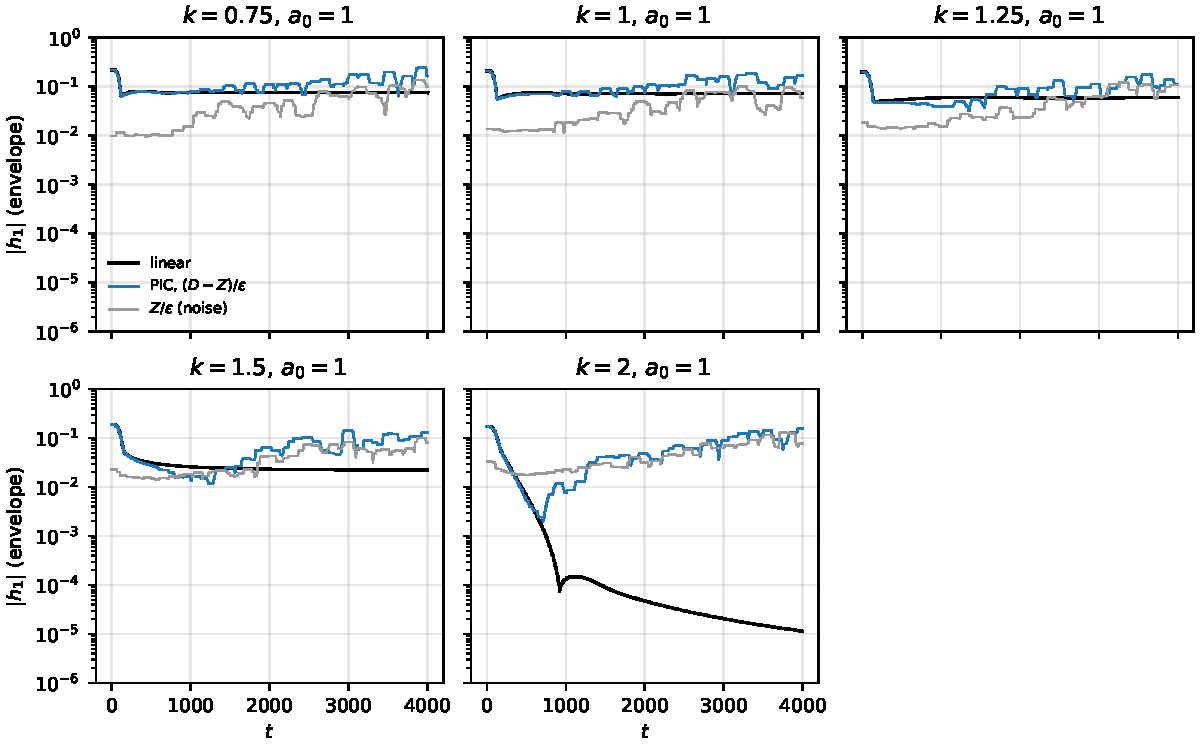
\includegraphics[width=\textwidth]{pic_a1.pdf}
\caption{$a_0=1$: envelope of $|h_1|$ in linear theory (black), in the PIC runs,
$(h_{1,D}-h_{1,Z})/\varepsilon$ (blue), and of the reference run alone, $h_{1,Z}/\varepsilon$ (grey),
which measures its departure from stationarity.}
\label{fig:a1}
\end{figure}

\begin{table}[!htbp]
\centering
\small
\begin{tabular}{lllrrrr}
\toprule
$k$ & $\omega_d$ ($\lambda=1$) & window & $\omega$ PIC & $\gamma$ PIC & $\omega$ linear & $\gamma$ linear\\
\midrule
0.75 & 0.14169 & 300--1500 & 0.14156 & $4\times10^{-5}$ & 0.14169 & $4\times10^{-6}$\\
1 & 0.14785 & 300--1500 & 0.14766 & $5\times10^{-5}$ & 0.14783 & $-1\times10^{-5}$\\
1.25 & 0.15326 & 300--1500 & 0.15326 & $4.1\times10^{-4}$ & 0.15330 & $1\times10^{-5}$\\
1.5 & 0.15751 & 300--1500 & 0.15805 & $1.5\times10^{-3}$ & 0.15736 & $1.0\times10^{-4}$\\
2 & -- & 100--600 & 0.16661 & $6.8\times10^{-3}$ & 0.16631 & $6.5\times10^{-3}$\\
\bottomrule
\end{tabular}
\caption{One-pole fits (matrix pencil, $M=3$) of $h_1$ at $a_0=1$, before the noise dominates.
The fits over $300$--$1000$ (and $100$--$400$ for $k=2$) give frequencies that differ by at most
$5\times10^{-4}$. For $k=1.25$ and $1.5$, $\gamma$ measures a dip of the amplitude, not a decay
(Section~\ref{sec:borde}).}
\label{tab:polos}
\end{table}

Table~\ref{tab:polos} and Figure~\ref{fig:a1} give the result.
\begin{itemize}
\item \textbf{$k=0.75$ and $k=1$ do not damp.} The PIC amplitude stays within \SI{10}{\%} of
the linear plateau up to $t\approx1000$, and the frequency agrees with $\omega_d$ to $9\times10^{-4}$ and
$1.3\times10^{-3}$ ($0.14156$ against $0.14169$, and $0.14766$ against $0.14785$).
\item \textbf{$k=2$ damps at the linear rate.} The fitted pole agrees with linear theory to
\SI{0.2}{\%} in $\omega$ and \SI{5}{\%} in $\gamma$, and the PIC amplitude follows the linear one down
by a factor of 40, until it reaches the noise at $t\approx600$.
\item \textbf{$k=1.25$ and $k=1.5$ lose amplitude.} The frequency is that of the discrete mode,
but the fitted pole has $\gamma=4\times10^{-4}$ and $1.5\times10^{-3}$, and the PIC amplitude is
\SIrange{14}{37}{\%} below the linear one at $t=500$--$1000$. These modes lie $0.019$ and $0.0015$
band widths below the edge. Section~\ref{sec:borde} shows that the loss is a finite-amplitude
effect, and that the mode of $k=1.25$ does not damp.
\item \textbf{The reference runs are not stationary at this mass.} $|h_{1,Z}|$ grows from $10^{-3}$
to $10^{-2}$ between $t=0$ and $4000$, and so does the noise of the subtraction. This limits the
comparison to $t\approx1000$--$1500$ (20--40 $\tau_1$, with $\tau_1=37$--$48$).
Section~\ref{sec:borde} separates the two causes.
\end{itemize}

\subsection{The modes next to the edge}
\label{sec:borde}

Series 4 tests the loss of the modes of $k=1.25$ and $1.5$. Each run changes one thing with
respect to the run of series 2: the amplitude ($\varepsilon=0.03$ and $0.3$, with the same
reference and the same particles), the grid ($\Delta r=0.05$ with the same $\Delta t=0.1$ and the
same initial state), or the number of particles ($800\times50=4\times10^4$, which also
doubles the resolution of the initial lattice in $J$ and $Q$). The last two have their own
reference. Table~\ref{tab:borde} gives the PIC amplitude relative to the linear one, and
Figure~\ref{fig:borde} the envelopes.

\begin{table}[!htbp]
\centering
\small
\begin{tabular}{llrrrrr}
\toprule
$k$ & run & $t=500$ & $1000$ & $2000$ & $3000$ & frequency, $t\ge2500$\\
\midrule
1.25 & $\varepsilon=0.03$ & 0.97 (0.91) & 1.21 (0.86) & 2.79 (1.33) & 4.66 (3.63) & 0.2210\\
 & $\varepsilon=0.1$ & 0.84 (0.27) & 0.66 (0.26) & 1.55 (0.40) & 1.05 (1.09) & 0.2179\\
 & $\varepsilon=0.3$ & 0.38 (0.09) & 0.47 (0.09) & 0.69 (0.13) & 0.48 (0.36) & 0.1531\\
 & $\Delta r/2$ & 0.88 (0.08) & 0.69 (0.23) & 1.44 (0.36) & 1.88 (1.26) & 0.1998\\
 & $4N$ & 0.84 (0.25) & 0.61 (0.24) & 0.81 (0.26) & 0.99 (0.27) & 0.1530\\
\midrule
1.5 & $\varepsilon=0.03$ & 1.02 (1.62) & 1.56 (2.56) & 6.69 (6.18) & 11.2 (12.4) & 0.2094\\
 & $\varepsilon=0.1$ & 0.86 (0.49) & 0.64 (0.77) & 2.39 (1.86) & 5.98 (3.71) & 0.2117\\
 & $\varepsilon=0.3$ & 0.34 (0.16) & 0.57 (0.26) & 1.83 (0.62) & 1.34 (1.24) & 0.2283\\
 & $\Delta r/2$ & 0.86 (0.13) & 0.80 (0.49) & 2.29 (1.18) & 3.89 (3.27) & 0.2075\\
 & $4N$ & 0.84 (0.49) & 0.41 (0.56) & 0.73 (0.63) & 1.34 (0.68) & 0.1584\\
\bottomrule
\end{tabular}
\caption{Envelope of $|h_1|$ (largest value in $[t,t+100]$) in the PIC runs divided by the
linear one, and in parentheses that of the reference run alone, $|h_{1,Z}|/\varepsilon$, divided
by the same linear value. The last column is the frequency of $h_1$ over $2500\le t\le4000$. In
linear theory it is $0.15325$ for $k=1.25$ and $0.15745$ for $k=1.5$; the band starts at
$\Omega_{\min}=0.15597$ and $0.15769$.}
\label{tab:borde}
\end{table}

\begin{figure}[htbp]
\centering
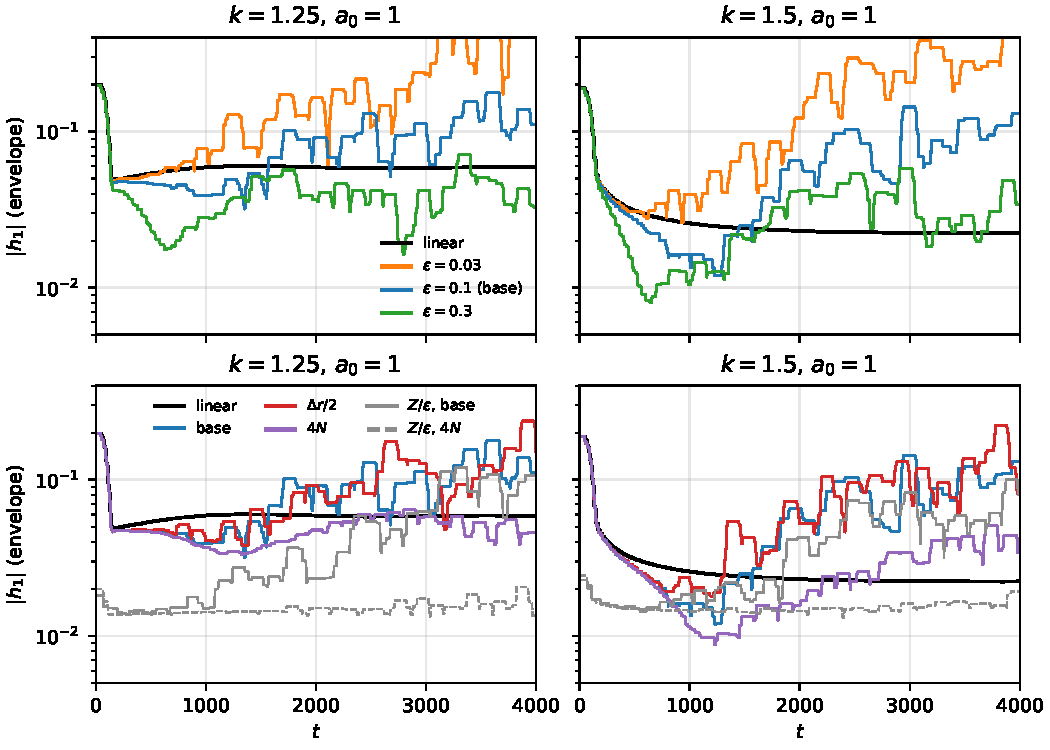
\includegraphics[width=0.9\textwidth]{pic_barrido.pdf}
\caption{Envelope of $|h_1|$ for $k=1.25$ (left) and $1.5$ (right) at $a_0=1$. Top: three
amplitudes with the same particles. Bottom: the run of series 2, the same with $\Delta r/2$ and
with four times more particles, and the reference runs alone, $|h_{1,Z}|/\varepsilon$ (grey), with
$10^4$ (solid) and $4\times10^4$ particles (dashed).}
\label{fig:borde}
\end{figure}

\begin{itemize}
\item \textbf{The loss is a finite-amplitude effect.} At $t=500$ the PIC amplitude is $0.97$,
$0.84$ and $0.38$ of the linear one for $\varepsilon=0.03$, $0.1$ and $0.3$ ($k=1.25$), and $1.02$,
$0.86$ and $0.34$ ($k=1.5$). With $\Delta r/2$ or $4N$ it is $0.84$--$0.88$, the value of
$\varepsilon=0.1$. Over $100\le t\le500$ the difference $|h_{1}(\varepsilon)-h_{1}(0.03)|$ is $3.6$--$7.1$
times larger for $\varepsilon=0.3$ than for $\varepsilon=0.1$; a correction to $h_1/\varepsilon$ linear
in $\varepsilon$ gives $3.9$ and a quadratic one $9.8$. Over the same interval, halving $\Delta r$ or
taking $4N$ changes $h_1$ by $2.8$--$13$ times less than going from $\varepsilon=0.03$ to $0.1$. The
demo found the same for its mode next to the edge (D3).
\item \textbf{The mode of $k=1.25$ does not damp.} With $4N$ the PIC amplitude is $0.6$--$1.0$
of the linear one up to $t=4000$, and $h_1$ oscillates at $0.1530$ ($\omega_d=0.15326$). With
$\varepsilon=0.3$ it falls to $0.38$ by $t=500$ and then stays at $0.5$--$0.9$, also at $0.1531$.
The $\gamma=4\times10^{-4}$ of Table~\ref{tab:polos} measures a dip of the amplitude, not a decay.
With $\varepsilon=0.1$ the amplitude reaches a minimum of $0.53$--$0.63$ of the linear one at
$t\approx1350$, with $10^4$ or $4\times10^4$ particles and with $\Delta r/2$, and with $4N$ it is back to
$1.0$ at $t=2500$. With $\varepsilon=0.3$ the minimum is deeper and earlier, $0.32$ at $t\approx630$. In
the run of series 2 the noise of the reference reaches the signal at $t\approx2500$ and hides
the recovery.
\item \textbf{The mode of $k=1.5$ is not resolved.} It lies $\Omega_{\min}-\omega_d=1.8\times10^{-4}$
below the edge, so it separates from the response of the edge only after
$t\sim1/(\Omega_{\min}-\omega_d)\approx5500$, longer than the runs; the linear solution itself still
decays at $t=4000$. With $4N$ the PIC amplitude is $0.4$--$0.7$ of the linear one for
$1000\le t\le2000$ and rises to $1.3$ by $t=3000$, at the frequency $0.1584$, while the noise of
the reference is $0.6$--$0.7$ of the linear amplitude. That is above
$\Omega_{\min}$, but the resolution of a window of 1500 is $2\pi/1500\approx4\times10^{-3}$. These runs
do not decide whether the mode survives.
\item \textbf{The departure of the references from stationarity has two causes}
(Table~\ref{tab:ruidoZ}). Up to $t\approx500$, $|h_{1,Z}|$ is $1.4$--$2.3\times10^{-3}$; with $\Delta r/2$
it is $2.5$--$4$ times less, and with $4N$ it does not change. This is the error of order
$\Delta r^2$ of the PIC field, which makes the initial state a slightly wrong equilibrium, as in
the demo (its Section~5.2). After $t\approx1000$, $|h_{1,Z}|$ grows to $10^{-2}$ by $t=3900$. With
$\Delta r/2$ the growth is the same, and with $4N$ it does not appear up to $t=4000$. This is the
discreteness of the particles, as for M5 in the demo.
\end{itemize}

\begin{table}[!htbp]
\centering
\small
\begin{tabular}{llrrrrrr}
\toprule
$k$ & reference & $t=0$ & $500$ & $1000$ & $2000$ & $3000$ & $3900$\\
\midrule
1.25 & $10^4$, $\Delta r=0.1$ & 1.8 & 1.5 & 1.5 & 2.3 & 6.4 & 11\\
 & $\Delta r/2$ & 0.72 & 0.44 & 1.4 & 2.1 & 7.4 & 12\\
 & $4N$ & 2.0 & 1.4 & 1.4 & 1.5 & 1.6 & 1.7\\
\midrule
1.5 & $10^4$, $\Delta r=0.1$ & 2.3 & 1.5 & 2.0 & 4.3 & 8.3 & 10\\
 & $\Delta r/2$ & 0.76 & 0.40 & 1.2 & 2.7 & 7.3 & 9.4\\
 & $4N$ & 2.4 & 1.5 & 1.4 & 1.4 & 1.5 & 1.9\\
\bottomrule
\end{tabular}
\caption{$|h_{1,Z}|$ of the reference runs at $a_0=1$, in units of $10^{-3}$ (largest value in
$[t,t+100]$).}
\label{tab:ruidoZ}
\end{table}

\section{Discussion}
\label{sec:discusion}

\paragraph{Established.}
\begin{itemize}
\item The criterion $\lambda_{\rm edge}>1$, the norm of the Mathur operator of [HRSS] at the edge
of the gap, reproduces their dichotomy at small mass: $\lambda_{\rm edge}\propto a_0$ for $k>1$
and $\lambda_{\rm edge}=\infty$ for $k\le1$.
\item At finite mass it gives the threshold that the theorem does not estimate:
$a_0\approx0.53$ for $k=1.25$, $a_0\approx0.93$ for $k=1.5$, above $1$ for $k\ge2$.
\item The time-domain linear solver agrees with the loop gain: plateaus at the frequency
$\omega_d$, to $4\times10^{-5}$ for $k\le1.25$, where $\lambda_{\rm edge}>1$, and damping where it is below
one.
\item The PIC runs reproduce the undamped modes of $k\le1$ and the damping of $k=2$ at $a_0=1$.
\item The loss of amplitude of the modes next to the edge in the PIC runs is a finite-amplitude
effect: it grows with $\varepsilon$ and does not change with $\Delta r$ or $N$. With $4\times10^4$
particles the mode of $k=1.25$ persists up to $t=4000$ at $\omega_d$.
\item The reference runs depart from stationarity for two reasons: the error of order $\Delta r^2$
of the PIC field sets the initial level, and the discreteness of the particles makes it grow
after $t\approx1000$. Four times more particles remove the growth up to $t=4000$.
\item $\eta$ does not mark the transition in this setting.
\end{itemize}

\paragraph{Open.}
\begin{itemize}
\item At small mass the discrete mode of $k\le1$ is bound by less than $10^{-6}$ band widths,
so a finite simulation sees only a slowly decaying edge response. The non-damping that the
theorem proves is not observable there; it becomes observable only at large mass.
\item The mode of $k=1.5$ at $a_0=1$, bound by $1.8\times10^{-4}$ in frequency. Deciding whether it
survives in the PIC runs needs $t\gtrsim10^4$ and the noise of $4N$ or less.
\item The dip of the amplitude of $k=1.25$. It is deeper and earlier with larger $\varepsilon$, but
whether it vanishes as $\varepsilon\to0$ is not measured: with $\varepsilon=0.03$ the noise reaches the
signal before the minimum. A run with $\varepsilon=0.03$ and $4N$ or more would measure it.
\item The noise floor at small mass, which limits the comparisons to $\sim10^3$ time units with
$10^4$ particles. Lowering it needs more particles; at $a_0=1$, $4\times10^4$ particles extend the
comparison to $t=4000$.
\end{itemize}

\section{Reproduction}
\label{sec:reproducir}

Everything is produced by \texttt{reproducir/scripts/hadzic.py} from that directory:
\begin{center}
\small
\begin{tabular}{lL{9.5cm}r}
\toprule
step & what it does & time\\
\midrule
\texttt{lineal} & the 36 equilibria, $\lambda_{\rm edge}$ (\texttt{exe/hadzic/lineal/lambda.txt}), $\eta$ (\texttt{eta.txt}) and the linear solutions of the runs & \SI{40}{min}\\
\texttt{preparar} & initial states and \texttt{.par} files in \texttt{reproducir/corridas/13\_hadzic/} & \SI{10}{min}\\
\texttt{correr} & the 34 PIC runs, one after another, with four threads & \SI{3.5}{h}\\
\texttt{analizar} & $h_1$ and $\delta\Phi$ in the map of the equilibrium, envelopes, slopes, pole fits and the table of series 4 (\texttt{exe/hadzic/resumen.txt}) & \SI{3}{h}\\
\texttt{figuras} & the figures of this report & \SI{1}{min}\\
\bottomrule
\end{tabular}
\end{center}
The runs of series 1 used the Courant factor 2 of the template, so they reached $t=8000$;
their \texttt{.par} files are kept as used, and their header comment says $t_{\rm fin}=4000$.
The runs with $\Delta r/2$ use the initial states of series 2; the dictionary \texttt{CAMBIOS} of the
script lists the changes of each run of series 4.

\section*{References}

\begin{itemize}
\item[{[HRSS]}] M.~Hadžić, G.~Rein, M.~Schrecker, C.~Straub, \emph{Damping versus oscillations
for a gravitational Vlasov--Poisson system}, Arch. Ration. Mech. Anal. 249:45 (2025),
\href{https://arxiv.org/abs/2301.07662}{arXiv:2301.07662}.
\item[{[HRS]}] M.~Hadžić, G.~Rein, C.~Straub, \emph{On the existence of linearly oscillating
galaxies}, Arch. Ration. Mech. Anal. 243 (2022), \href{https://arxiv.org/abs/2102.11672}{arXiv:2102.11672}.
\item[{[S]}] C.~Straub, \emph{Numerical experiments on stationary, oscillating, and damped spherical
galaxy models}, \href{https://arxiv.org/abs/2405.01235}{arXiv:2405.01235} (2024).
\end{itemize}
The other works of the group and the comparison of their setting with ours are in
\texttt{docs/hadzic/hadzic\_base.md}.

\end{document}
